% This is LLNCS.DEM the demonstration file of
% the LaTeX macro package from Springer-Verlag
% for Lecture Notes in Computer Science,
% version 2.4 for LaTeX2e as of 16. April 2010
%
\documentclass{llncs}
%
%\usepackage{makeidx}  % allows for indexgeneration
\usepackage{parskip}
\usepackage{wrapfig}
\usepackage{array}
\usepackage{float}
\usepackage[english]{babel}
\usepackage{lipsum}
\usepackage{caption}
\usepackage{subcaption}
\usepackage{graphicx}
\graphicspath{{images/}} 
%\usepackage{cite}
\usepackage[linesnumbered,ruled]{algorithm2e}
\usepackage{courier}
\usepackage{hyperref}
\hypersetup{colorlinks=true,allcolors=blue}
\usepackage{listings}
\lstset{
    basicstyle=\ttfamily,
    frame=none, 
    breaklines=true,
    numbers=left,
    xleftmargin=2.5em,
    framexleftmargin=0em,
    emphstyle=\textbf,
    float=t
}
\lstdefinestyle{ocl}{
    emph={
context, inv
    }
}
\lstdefinestyle{cbp}{
    basicstyle=\ttfamily\scriptsize,
    emph={
session, create, of, type,
set, to, add, hire
    }
}
\lstdefinestyle{xmi}{
    basicstyle=\ttfamily\scriptsize,
    emph={
Node, children
    }
}
\lstdefinestyle{xml}{
    basicstyle=\ttfamily\scriptsize,
    emph={
register, create, add, to, resource,
from, eattribute, remove, ereference,
set, unset, session, Roy, Jen,
Moss, Richmond
    }
}
\lstdefinestyle{java}{
    basicstyle=\ttfamily\scriptsize,
    emph={
case, UNSET,
instanceof, else, if, void,
new, UnsetEAttributeEvent,
UnsetEReferenceEvent,
@override, public, class, extends
    }
}
\lstdefinestyle{eol}{
    basicstyle=\ttfamily\scriptsize,
    emph={
var, new, for, in, create, set, of, with, 
unset, to, add, remove, delete, register, move,
from, position, from, move-within, session, \.
    }
}

\begin{document}
    \renewcommand{\thelstlisting}{\arabic{lstlisting}}
    \renewcommand{\labelitemi}{$\bullet$}
    \newcommand{\dk}[1]{\textbf{[DK: #1]}}
    
    \title{An Efficient Loading \\ of Change-Based Models}
    %
    %\titlerunning{An Efficient Loading of Change-Based Models}  % abbreviated title (for running head)
    %     also used for the TOC unless
    %     \toctitle is used
    %
    \author{
anonym%Alfa Yohannis \and Horacio Hoyos Rodriguez \and Fiona Polack$^*$ \and Dimitris Kolovos
    }
    %
    \authorrunning{
Anonym%Alfa Yohannis et al.
    } % abbreviated author list (for running head)
    %
    %%%% list of authors for the TOC (use if author list has to be modified)
    %\tocauthor{Alfa Yohannis,Horacio Hoyos Rodriguez, Fiona Polack, Dimitris Kolovos}
    %
    
    \institute{anonym}
    %\institute{Department of Computer Science, University of York, United Kingdom\\$^*$School of Computing and Maths, Keele University, United Kingdom\\
    %\email{\{ary506, horacio.hoyos, dimitris.kolovos\}@york.ac.uk\\$^*$f.a.c.polack@keele.a.cuk}}
    
    \maketitle      % typeset the title of the contribution
    %The first states the problem. The second states why the problem is a problem. The third is my startling sentence. The fourth states the implication of my startling sentence.
    \begin{abstract}
This paper proposes and evaluates an efficient approach for loading models stored in a change-based format. The work builds on language-independent change-based persistence (CBP) of models conforming to object-oriented metamodelling architectures such as MOF and EMF, an approach which persists a model's editting history rather than its current state. We evaluate the performance of the new loading approach  and assess its impact on saving change-based models. Our results show that the proposed approach significantly improves loading times compared to the baseline CBP loading approach, and has negligible impact on saving.


    \end{abstract}
    
    \section{Introduction}
    \label{sec:introduction}
    Conventional approaches for file-based model persistence in metamodelling architectures such as MOF \cite{omg2018mof} and EMF \cite{steinberg2008emf} are state-based -- saving the current state of a model.  In these approaches,  version control and change detection are delegated to external systems.  State based persistence is computationally expensive, as a whole model must be saved and loaded; this particularly effects large models and collaborative developments.
    
    In \cite{yohannis2017turning}, Yohannis et al. proposed change-based persistence (CBP), an approach that persists the full sequence of \emph{changes} made to a model instead of persisting the state.  Compared to the state-based approach, CBP supports fast detection of change, which speeds up model comparison and merging, as well as fast incremental model validation and transformation \cite{rath2012derived,ogunyomi2015property}.
    However, saving the change history of a model results in large, and growing, CBP files.  Loading times are also significant, as the load has to reconstruct a model's current state from its history\cite{yohannis2017turning}.   This paper proposes and evaluates an approach that reduces CBP model loading time by avoiding the replaying of changes that have no impact on the current state of the model.
    
    The rest of the paper is structured as follows. Section \ref{sec:case_study} introduces a running example and provides a brief introduction to CBP.
    Section \ref{sec:loading_time_optimisation} presents the approach to speed up model loading and its supporting data structures. Section \ref{sec:complexity_analysis} discusses the time complexity of our approach. Section \ref{sec:performance_evaluation} presents experimental results and evaluation. Section \ref{sec:related_work} provides an overview of related work, and Section \ref{sec:conclusions} concludes with discussion of directions for future work.
    
    \section{Running Example}
    \label{sec:case_study}
    To explain model CBP, we use the minimal tree metamodel and an example tree model, Figures \ref{fig:tree_metamodel} and \ref{fig:initial_model}.
    The metamodel is expressed the Eclipse Modelling Framework (EMF) Ecore metamodelling language, the de-facto standard for object-oriented metamodelling.  The example is contrived to avoid unnecessary repetition, whilst providing adequate coverage of the core features of Ecore (classes, single/multi-valued features, references).
    In this example, a tree model consists of named nodes which can -- optionally -- contain other nodes (\emph{child} references).
    
    \begin{figure}[ht]
\begin{subfigure}[t]{0.4\linewidth}
    \centering
    \includegraphics[width=0.8\linewidth]{node_metamodel}
    \caption{The tree metamodel (EMF/Ecore).}
    \label{fig:tree_metamodel}
\end{subfigure}
\hfill
\begin{subfigure}[t]{0.6\linewidth}
    \centering
    \includegraphics[width=0.6\linewidth]{initial_chart}
    \caption{A tree model that conforms to the  metamodel.  Node n3 is created and then deleted.}
    \label{fig:initial_model}
\end{subfigure}
\caption{Running example of a metamodel and a conformant model.}
\label{fig:append_speed}
    \end{figure}
    
    The current state of the model in Fig. \ref{fig:initial_model} has two nodes, \emph{n1}, \emph{n2}.  The model was constructed in a series of steps.  First, three nodes were created (\emph{n1}, \emph{n2} and \emph{n3}).
    Nodes \emph{n2} and \emph{n3} were then added as children of \emph{n1}.
    Finally, node \emph{n3} was deleted.
    
    Listings \ref{lst:xmimodel} shows the state-based representation of the current model, using simplified XML.  Listing \ref{lst:cbpmodel} shows the change-based representation, using the CBP syntax introduced in \cite{yohannis2017turning}.
    
    \noindent
    \begin{minipage}[t]{0.5\linewidth}
\begin{lstlisting}[style=xmi,caption={State-based tree model.},label=lst:xmimodel]
<Node id="n1" name="A">
<children id="n2" name="B"/>
</Node>
\end{lstlisting}
    \end{minipage}
    \hfill
    \begin{minipage}[t]{0.5\linewidth}
\begin{lstlisting}[style=eol,caption={Change-based tree model.},label=lst:cbpmodel]
create n1 of Node
set n1.name to "A"      
create n2 of Node
set n2.name to "B"      
create n3 of Node
set n3.name to "C"      
add n2 to n1.children   
add n3 to n1.children
remove n3 from n1.children   
delete n3
\end{lstlisting}
    \end{minipage}
    
    Lines 1-6 of Listing \ref{lst:cbpmodel} 
    record the creation and naming of the three nodes; lines 7-8 record the addition of \emph{n2} and \emph{n3} as children of \emph{n1}; lines 9-10 capture the deletion of \emph{n3} ('remove'   represents the removal of an element from its container; 'delete' completely removes an element from its model).
    
    The example model history illustrates a case where  earlier events (creating \emph{n3} in line 5, naming it in line 6, making it a child of \emph{n1} in line 8, removing it from the container in line 9) are superseded by a subsequent event (deletion of \emph{n3} in line 10).  Loading of the current model would be faster if the events in lines 5, 6, 8, 9 and 10 could be ignored.
    
    \section{Towards Efficient Loading of Change-Based Models}
    \label{sec:loading_time_optimisation}
    The flowchart in Fig. \ref{fig:flowchart} provides an overview of the editing lifecycle of a CBP model \cite{yohannis2017turning}, with the proposed extensions shown as starred blocks.  A model is loaded, edited and saved.  During editting, the "change events" that change the model are recorded in a memory-based data structure, serialised and with the latest event appended at the end.  The change events are flushed from memory (persisted: the CBP file) every time the model is saved.  When a model is re-loaded, the current model state is recreated from the saved CBP file.
    
    \begin{figure}[ht]
\centering
\includegraphics[width=\linewidth]{flowchart}
\caption{CBP workflow, with optimised loading elements indicated by starred blocks.}
\label{fig:flowchart}
    \end{figure}

    A key principle of CBP is that all events are saved.  Compression, to remove superseded events, cannot be applied to the persisted file directly.  Therefore, the proposed approach adds two artefacts: a ``Model History'' data structure which is populated with change events and which is used to detect superseded events prior to saving, and an ``Ignore List'' file, which persists the position (i.e. line numbers) of superseded events so that they can be ignored the next time the model is loaded.  The Ignore List is saved, with the CBP file.
    
    \subsection{Model History}
    \label{subsec:model_history}
    The Model History data structure stores events and their line number in a CBP representation.  The data can be used to reason about the events of a particular element and to determine which events are superseded.  We refer to the line number in the CBP representation as the \emph{event number}.
    The proposed data structure is defined in Fig. \ref{fig:object_history} using a class diagram.  
     
    A \emph{ModelHistory} has a \emph{URI} attribute to identify the model for which it records changes.  A \emph{ModelHistory}  can link to many \emph{ElementHistory} objects, each identified by its \emph{element} field. 
    An \emph{ElementHistory} can link to many \emph{FeatureHistories}, representing the editing histories of individual features -- either references or attributes) of the element. 
    A \emph{FeatureHistory} has a \emph{type} (attribute or reference) and a \emph{name}, identifying the feature.
    
     \begin{figure}[ht]
\centering
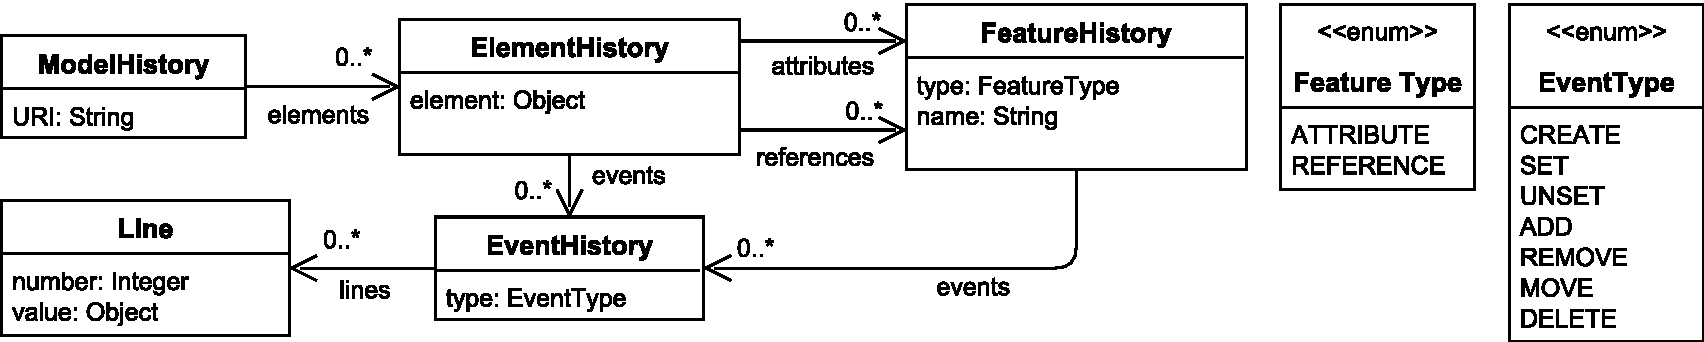
\includegraphics[width=\linewidth]{object_history}
\caption{The class model defining Model History.}
\label{fig:object_history}
    \end{figure}

     \begin{figure}[ht]
\centering
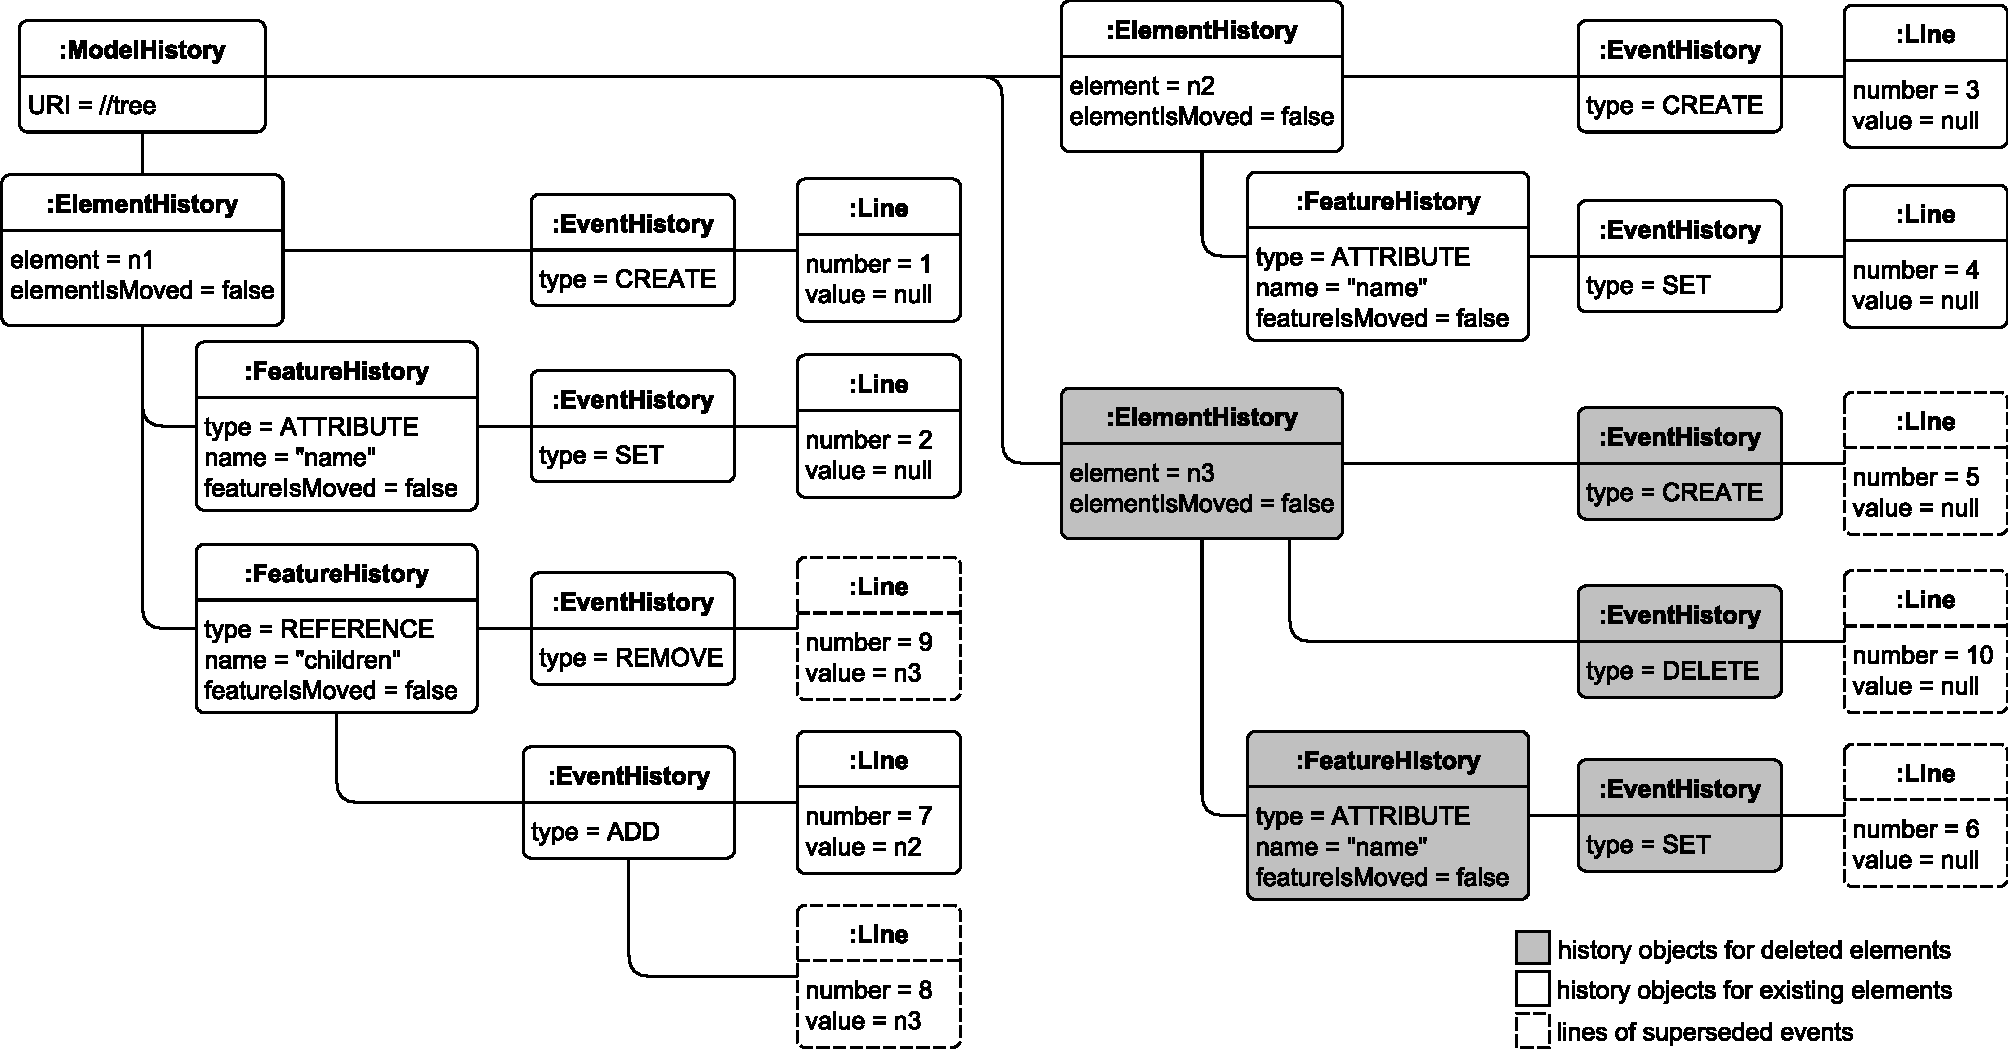
\includegraphics[width=\linewidth]{history_structure}
\caption{The object diagram of the CBP model history in Listing \ref{lst:cbpmodel}.}
\label{fig:history_structure}
    \end{figure}
    
    
    An \emph{EventHistory} represents series of events of the same type; it has an attribute \emph{type} to identify the events' type, and can have many \emph{Line}s.  A \emph{Line} has a \emph{number} attribute, to record the event number, and a \emph{value} that records the element involved in the event (Value is only used for \emph{ADD}, \emph{REMOVE} and \emph{MOVE} events). Each \emph{FeatureHistory} can have many \emph{EventHistories}, to represent the events that modify the values of the features.
    Each \emph{ElementHistory} can have many \emph{EventHistories} to represent events that affect the state of the elements (life-cycle and relations to multivalued features).
    
    Fig. \ref{fig:history_structure} shows an object diagram corresponding to the model in Fig. \ref{fig:object_history} that captures the model history shown in Listing \ref{lst:cbpmodel}. The grey rectangles are \emph{History} objects related to the deleted node \emph{n3}. The rectangles with the dashed outline are \emph{Line} objects that represent superseded changes. 
      
    The generic identification of superseded events relies on various strategies.  We now present strategies we use to create the Ignore List for a CBP model. 

    \subsection{Set and Unset Events}
    \label{subsec:set_and_unset_operations}
    During the lifecycle of a model, a single-valued feature can have a value set (assigned) or unset many times.  Each event is persisted, but only the last assigned value needs to be considered. For example, in Listing \ref{lst:set_unset_example_1}, the feature \emph{name} is set to the value ``A'', unset, and finally set to the value ``B''.  In the current state of the model, \emph{n1.name} = ``B'', and the model loading activity can thus ignore the change events on lines 2 and 3. 
    
    \noindent
    \begin{minipage}[t]{0.49\linewidth}
\begin{lstlisting}[style=eol,caption={A CBP representation of attribute \emph{name} assignments.},label=lst:set_unset_example_1]
create n1 of Node
set n1.name to "A"
unset n1.name
set n1.name to "B"
\end{lstlisting}
    \end{minipage}
    \hfill
    \begin{minipage}[t]{0.49\linewidth}
\begin{lstlisting}[style=eol,caption={A CBP representation of attribute \emph{name} assignments.},label=lst:set_unset_example_2]
create n1 of Node
set n1.name to "A"
set n1.name to "B"
unset n1.name
\end{lstlisting}
    \end{minipage}
    
    Based on the Listing \ref{lst:set_unset_example_1}, our approach creates an instance of $ElementHistory$ $n1$ which contains an instance of $FeatureHistory$ $name$. The $FeatureHistory$ $name$ consists of two $EventHistory$ instances, with types \textit{SET} and \textit{UNSET} (the instances are named $set$ and $unset$ respectively for brevity). The $set$ records the $Line$ instances that hold the the event numbers where the \textit{SET} events, and similarly for $unset$.
    
    From Listing \ref{lst:set_unset_example_1}, we can thus infer that $name$.$set$.$lines$ = $\{2,4\}$ and $name$.$unset$. $lines$ = $\{3\}$. The event numbers in both lists are used to determine that the events represented by lines 2 and 3 are superseded by that in line 4, which is a $set$ event, giving an $ignoreSet$ = $\{2, 3\}$.  By the same process, for Listing \ref{lst:set_unset_example_2}, we can reason that $name$.$set$.$lines$ = \{2,3\} and $name$.$unset$.$lines$ = \{4\}.  However, this case, the highest-numbered event is an $unset$, so line numbers are put into the $ignoreSet$ ($ignoreSet$ = $\{2, 3, 4\}$). In general, an \textit{UNSET} event can be ignored along with all preceding \textit{SET} and \textit{UNSET} events. 
    
    \subsection{Add, Remove, and Move Events}\label{subsec:add_remove_and_move_operations}
    For a multi-valued feature, events add, remove and move can be called many times, to modify the feature. If an element is added to the feature, moved multiple times, and finally removed, then all the element's preceding events can be ignored. 
    
    For example, in Listing \ref{lst:add_remove_move_reference},  nodes $n1$, $n2$, and $n3$ are added to the $children$ feature of $p$ (lines 5-7), then $n3$ is moved to index 1 (where index starts from 0), $n1$ is moved to index 2 (line 9), $n3$ is moved to index 2 (line 10), and finally $n3$ is removed (line 11).  In the latest state of the model, $children$ only contains $n1$ and $n2$. As a result, the loading process could ignore the events that represent the \textit{ADD}, \textit{MOVE}, and \textit{REMOVE} events on $n3$. 
    
    To create the Ignore List for the Listing \ref{lst:add_remove_move_reference}, we can deduce that $children$.$add$. $lines$ = \{\{5, $n2$\}, \{6, $n3$\} \{7, $n3$\}\} (5 is the line number and $n2$ is the value); $children$.$move$.$lines$ = \{\{8, $n3$\}, \{9, $n1$\}, \{10, $n3$\}\}; and $children$.$remove$.$lines$ = \{$n$3\}. Since $n3$ is removed from its containing feature (line 11), then executing its preceding add and remove events is unnecessary. Note that we retain the \textit{create} event (line 4) as $n3$ has not been deleted.  We can iterate through the add, remove and move structures to identify the events on $n3$ that should be removed, resulting in the $ignoreSet$ = \{7, 8, 10, 11\}
    
\noindent
    \begin{minipage}[t]{0.48\linewidth}
\begin{lstlisting}[style=eol,caption={A CBP representation of add, move, and remove operations.},label=lst:add_remove_move_reference]
create p of Node
create n1 of Node
create n2 of Node
create n3 of Node
add n1 to p.children
add n2 to p.children
add n3 to p.children
move n3 to 1 in p.children  
move n1 to 2 in p.children  
move n3 to 2 in p.children
remove n3 from p.children   
\end{lstlisting}
    \end{minipage}
    \hfill
    \begin{minipage}[t]{0.48\linewidth}
\begin{lstlisting}[style=eol,caption={The optimised CBP representation of Listing \ref{lst:add_remove_move_reference}},label=lst:optimised_add_remove_move_reference]
create p of Node
create n1 of Node
create n2 of Node
create n3 of Node
add n1 to p.children
add n2 to p.children  
move n1 to 2 in p.children
\end{lstlisting}
    \end{minipage}
    
    
    \subsection{Create and Delete Events}
    \label{subsec:create_and_delete_operations}
    
    When an element is deleted, it is completely removed from the model. Therefore, all previous events (create, set, unset, move, add, remove, delete) on that element can be ignored, along with all events on the element's features. 
    
    For example, when node \emph{n3} in Listing \ref{lst:cbpmodel} is deleted, the events in lines 5-6 and 8-10 are superseded. The optimised change-based representation of Listing \ref{lst:cbpmodel} is presented in Listing \ref{lst:cbpmodel_optimised}.
    
    \begin{lstlisting}[style=eol,caption={Change-based representation of the model in Fig. \ref{fig:initial_model} after removal of node \emph{n3}.},label=lst:cbpmodel_optimised]
create n1 of Node
set n1.name to "A"
create n2 of Node
set n2.name to "B"
add n2 to n1.children
    \end{lstlisting}
    
    Using the Listing \ref{lst:cbpmodel}, we can construct the structure of histories that are related to element $n3$ as follows: $n3$.$create$.$lines$ = \{5\}, $n3$.$name$.$set$.$lines$ = \{6\}, $n1$.$children$.$add$.$lines$ = \{\{7, $n2$\}, \{8, $n3$\}\}, $n1$.$children$.$remove$.$lines$ = \{\{9, $n3$\}\}, and $n3$.$delete$.$lines$ = \{10\}. Thus, when element $n3$ is deleted, by iterating through all these history structures, all line numbers associated with $n3$ can be identified and added to $ignoreSet$ producing $ignoreSet$ = \{5 6, 8, 9, 10\} so they can be ignored in the next model loading.
    
    \section{Execution Time Analysis}
    \label{sec:complexity_analysis}
    
    In this section, we analyse the execution time of the original and optimised CBP approaches, to determine theoretically how they differ in terms of loading models and persisting changes.   
    
    \subsection{Time for Loading Models}
    
    The optimised loading of a CBP model executes Algorithm \ref{alg:load}.  The algorithm takes two inputs: a CBP file $cbpFile$ and an Ignore Set $ignoreSet$. After initialisation of structures, the algorithm iterates through all the lines of the $cbpFile$ using the $readLine$ method, and assigns each line to the $line$ variable. Each iteration checks whether the $event$'s $lineNumber$ exists in the $ignoreSet$ using the $contains$ method (the $ignoreSet$ is implemented in HashSet which only has $O(1)$ complexity for search).  If $contains$ is  $true$ then the algorithm iterates to the next line, but if $contains$ is  $false$ then the $line$ is parsed using the $parseToEvent$ function to produce an $event$ to be replayed. Otherwise, it just continues to the next iteration. 
      
    To calculate time complexity, we need to consider the data as well as the algorithm.  Every CBP model is represented as a set of event line numbers (the CBP file), $E$ = \{$e_1$, $e_2$, ... $e_n$\}, where $E$ is the set, $e_1$, $e_2$, ... $e_n$ is a line number.  The size of $N$ = $|E|$. The representation also has an $ignoreSet$ that contains line numbers that will not be replayed when loading the model. The $ignoreSet$ is denoted as a set $I$  = \{$i_1$, $i_2$, ... $i_m$\}, such that $I$ is the $ignoreSet$, $i_1$, $i_2$, ... $i_m$ are the ignored line numbers, and $M$ is the size of $I$, $M$ = $|I|$. Also, $I$ $\subseteq$ $E$, indicating that the $I$ cannot contain a line number that does not exist in $E$.
    
    Let us assume that the total time to complete running of all the events is $T_E$ = $t_1$ + $t_2$ + ... + $t_n$, such that $t_1$, $t_2$, ... $t_n$ are the times required for completing each event. If we assume that the time required to finish executing an event is the same for each event, $t_c$, then $T_E$ = $N$ $\times$ $t_c$.  By the same reasoning, the total time saved by ignoring superseded events,  $T_I$ = $t_1$ + $t_2$ + ... + $t_m$; if $t$ is constant for all the events then $T_I$ = $M$ $\times$ $t_c$.
    
    \IncMargin{1.5em}
    \begin{algorithm}[H]
\begin{small}
    \SetKwInOut{Input}{input}
    \SetKwInOut{Output}{output}
    \Input{a CBP file $cbpFile$, an Ignore Set $ignoreSet$}
    \Begin{
initialise()\;
$lineNumber$ $\leftarrow$ 1\;
\While{($line$ $\leftarrow$ cbpFile.readLine()) != $null$}{
    \uIf{ignoreSet.contains($lineNumber$) $!=$ $true$ }{
$event$ $\leftarrow$ parseToEvent($line$)\;
replay($event)$\;
    }
    $lineNumber$ $\leftarrow$ $lineNumber$ + 1\;
}
finalise()\;
    }
\end{small}
\caption{Algorithm for optimised CBP model loading.}
\label{alg:load}
    \end{algorithm}
    \DecMargin{1.5em}

    The unoptimised CBP loading time, is the time required to load a model: $T_T$ = $T_E$ + $T_O$, where $T_O$ is the total time needed to complete other required routines (represented by the $initialise()$, $readLine()$, and $finalise()$ routines in Algorithm \ref{alg:load}). For optimised CBP loading, the total time to load an change-based model is reduced by the total time saved-up by ignoring superseded events, that is $T_T$ = $T_E$ + $T_O$ $-$ $T_I$. In the worst case, there is no event that is ignored, $T_T$ = $T_E$ + $T_O$ $-$ 0. In the best case, all events are ignored, $T_T$ = $T_E$ + $T_O$ $-$ $T_E$ = $T_O$. The $T_O$ time can be reduced by using faster reading methods and more efficient formats of CBP representation. 
    
    Loading a state-based model should be faster than loading a change-based model. Loading a state-based model only requires to read the the model from its representation and transform it into a model in memory; there is no need to parse and replay persisted events.
    
    \subsection{Time for Persisting Changes}
    Algorithm \ref{alg:save} outlines the persisting of a CBP model. All events raised from modifying the model are recorded into an $eventList$. When a user saves the model, the algorithm starts by initialising an empty set, $ignoredLineNumbers$. It then iterates through all the $events$ in the $eventList$ and adds the event into a $ModelHistory$ using $addEventToModelHistory$.  The strategies outlined in Sections \ref{subsec:set_and_unset_operations}--\ref{subsec:create_and_delete_operations} are encoded in  $addEventToModelHistory$, and are executed to identify superseded events. The line number of each superseded events is written to  $ignoredLineNumbers$ and the event is then parsed into a string $line$ and appended into a $cbpFile$, using the $parseToLine$ and $append$ methods. The algorithm ends by appending all the ignored line numbers to the (existing) $ignoreSet$ using the $append$ method.
    
    \IncMargin{1.5em}
    \begin{algorithm}[H]
\begin{small}
    \SetKwInOut{Input}{input}
    \SetKwInOut{Output}{output}
    \Input{a list of Event $eventList$, a CBP File $cbpFile$, an Ignore Set $ignoreSet$}
    \Begin{
$ignoredLineNumbers$ $\leftarrow$ \{\}\;
\ForEach{$event$ in $eventList$}{
    addEventToModelHistory($event$, $ignoredLineNumbers$)\;
    $line$ $\leftarrow$ parseToLine(event)\;
    $cbpFile$.append($line$)\;
}
\ForEach{$lineNumber$ in $ignoredLineNumbers$}{
    $ignoreSet$.append($lineNumber$)\;
}
    }
\end{small}
\caption{Algorithm for persisting changes of CBP.}
\label{alg:save}
    \end{algorithm}
\DecMargin{1.5em}
    
    Suppose that when a model is modified,  $N$ events are generated, of which $M$ are identified as ignored events. The total time to persist the change is $T_T$ = ($N$ $\times$ $T_E$) + ($M$ $\times$ $T_{AI}$) + $T_O$, where $T_E$ is the time to append an event to a $cbpFile$, $T_{AI}$ is the time to append a number to an $ignoreSet$, and $T_O$ is the time used for other required routines. The value of $T_E$ = $T_{MH}$ + $T_P$ + $T_{AC}$, where $T_MH$ is the sum of the time for adding the event to a model history and identifying ignored line numbers, $T_P$ is the time for parsing the $event$ to a string $line$, and $T_{AC}$ is the time for appending the $line$ to the $cbpRepresentation$. Thus, $T_T$ = ($N$ $\times$ ($T_{MH}$ + $T_P$ + $T_{AC}$))  + ($M$ $\times$ $T_AI$) + $T_O$. 
    
    For unoptimised CBP, persisting changes does not involve model history and ignore set therefore $T_{MH}$ and $T_AI$ can be ignored yielding $T_T$ = ($N$ $\times$ ($T_P$ + $T_{AC}$)) + $T_O$, implying that persisting changes in the original CBP should be faster than the optimised CBP. 
    
    Compared to saving a large state-based model, persisting small changes using CBP is much faster, since only the generated events  are persisted, not the entire model. In the best case, only one new event line is appended. In the worst case, a model is changed many times but is then largely deleted -- persisting many events but only a small-size model is saved. 
    
    %\textbf{*** NOTE: time complexity is not exactly the same as execution time...   This is not a complexity analysis!!!  Talk to D and H and sort terminology. Fiona}
    
    \section{Performance Evaluation}
    \label{sec:performance_evaluation}
    
    We developed the proposed efficient loading approach on top of the original CBP implementation\footnote{The prototype and the tests used in the evaluation are available under [hidden for review] for reproducibility. %\url{https://github.com/epsilonlabs/emf-cbp}
    } from \cite{yohannis2017turning} and evaluated our approach's model loading performance, as well as its memory footprint and its impact on the time required to save changes made to CBP models. The evaluation was performed on Intel\textsuperscript{\textregistered} Core\textsuperscript{TM} i7-6500U CPU@2.50GHz 2.59GHz, 12GB RAM, and the Java\textsuperscript{TM} SE Runtime Environment (build 1.8.0\textunderscore162-b12).
    
    Given that CBP is a very recent contribution and we are not aware of any existing datasets containing real-world models expressed in a change-based format, we have used synthetic change-based models for the evaluation of our experiments. The synthetic models were derived from real-world cases: the BPMN2 \cite{eclipse2017bpmn2,eclipse2018bpmn2git} and Epsilon \cite{eclipse2017epsilon,eclipse2018epsilongit} software projects, and the article on the United States \cite{wikipedia2018us} on Wikipedia. For the first two projects, for each version of the cases, we used MoDisco \cite{DBLP:journals/infsof/BruneliereCDM14} to generate a model that conforms to the UML2 \cite{eclipse2017uml2} metamodel.  For the States article, a model that conforms to the Modisco XML metamodel \cite{eclipse2018modiscoxml} is generated. A change-based model for each case is derived by comparing an initially-empty running model to different versions of the case's models sequentially. All identified differences are then reconciled by performing a unidirectional merging to the running model. All changes made to the running model during the merging process were captured and persisted into a CBP file. We use EMF Compare \cite{eclipse2017compare} to perform the comparison and merging.
    
    \begin{table} [ht]
\centering
\caption{Description of change-based models generated for evaluation.}
\label{table:data_description}
\begin{tabular}{|>{\centering\arraybackslash}p{1.5cm}|>{\centering\arraybackslash}p{1.7cm}|>{\centering\arraybackslash}p{2.4cm}|>{\centering\arraybackslash}p{1.6cm}
|>{\centering\arraybackslash}p{1.5cm}|>{\centering\arraybackslash}p{2cm}|}
    \hline 
    \textbf{Model} & \textbf{Total Events} & \textbf{Ignored Events} & \textbf{Elements} & \textbf{Total Versions} & \textbf{Processed Versions} \\
    \hline
    BPMN2 & \multicolumn{1}{r|}{1,238,752} & \multicolumn{1}{r|}{1,078,058 (87\%)} & \multicolumn{1}{r|}{62,062} & \multicolumn{1}{r|}{192} & \multicolumn{1}{r|}{192 (100\%)} \\
    \hline
    Epsilon & \multicolumn{1}{r|}{1,700,855} & \multicolumn{1}{r|}{1,433,147 (84\%)} & \multicolumn{1}{r|}{48,625} & \multicolumn{1}{r|}{3,037} & \multicolumn{1}{r|}{373 (12\%)} \\
    \hline 
    Wikipedia & \multicolumn{1}{r|}{10,496,645} & \multicolumn{1}{r|}{7,169,001 (68\%)} & \multicolumn{1}{r|}{11,849} & \multicolumn{1}{r|}{37,996} & \multicolumn{1}{r|}{2,973 (8\%)} \\
    \hline 
\end{tabular}
    \end{table}
    
    Table \ref{table:data_description} summarises events, elements and saved versions for the Epsilon, BPMN2, and Wikipedia cases. Total Events is the numbers of events that were produced by our approach in generating a change-based model for each case.  Ignored events is the number of superseded events that do not need to be replayed when reloading the models. Elements is the number of elements contained in each model. Total versions is the number of commits/revisions made to the cases, taken from the git repositories or Wikipedia at the time this evaluation performed. Processed versions is the number of commits/revisions that were processed to produce change-based models: since the comparison between versions takes considerable time, not all versions are processed here. 
    
    \subsection{Model Loading Time}
    \label{subsec:loading_time_test}
    
    \begin{figure}[ht]
\begin{subfigure}{0.325\textwidth}
    \centering
    \includegraphics[width=\linewidth]{images/load_time_bpmn2}
    \caption{BPMN2}
    \label{fig:load_time_bpmn2}
\end{subfigure}
\hfill
\begin{subfigure}{0.325\textwidth}
    \centering
    \includegraphics[width=\linewidth]{images/load_time_epsilon}
    \caption{Epsilon}
    \label{fig:load_time_epsilon}
\end{subfigure}
\hfill
\begin{subfigure}{0.325\textwidth}
    \centering
    \includegraphics[width=\linewidth]{images/load_time_wikipedia}
    \caption{United States}
    \label{fig:load_time_wikipedia}
\end{subfigure}
\caption{Results for loading a model in CBP, optimised CBP (OCBP), and for loading a state-based (XMI) representation (See Table \ref{table:ttest_results} for the t-test results).}
\label{fig:loadtime}
    \end{figure}
    
    To compare performance, we ran the optimised and unoptimised (baseline) CBP algorithms to reconstruct the current state of each of the three  models. The results are shown in Fig. \ref{fig:loadtime}.  These loading times show a considerable time saving for optimised CBP: BPMN2 was 56\% faster; Epsilon 50\% faster, and the United States page 36\% faster than in the original CPB implementation.
    
    For reference, we also compare CBP loading with the execution time for loading the equivalent state-based model in XMI. Fig. \ref{fig:loadtime} shows that, even with the improvements delivered by the new algorithm, loading change-based models is still significantly slower than loading a state-based model.  
    
    As discussed in\,\cite{yohannis2017turning}, CBP loading time penalties are balanced against the benefits that CBP brings, in terms of quicker, more precise differencing and more efficient incremental execution of model management programs.
    
    \subsection{Model Saving Time}
    \label{subsec:saving_time_test}
    
    
    
    \begin{figure}[ht]
\begin{subfigure}{0.325\textwidth}
    \centering
    \includegraphics[width=\linewidth]{images/save_time_bpmn2}
    \caption{BPMN2}
    \label{fig:save_time_bpmn2}
\end{subfigure}
\hfill
\begin{subfigure}{0.325\textwidth}
    \centering
    \includegraphics[width=\linewidth]{images/save_time_epsilon}
    \caption{Epsilon}
    \label{fig:save_time_epsilon}
\end{subfigure}
\hfill
\begin{subfigure}{0.325\textwidth}
    \centering
    \includegraphics[width=\linewidth]{images/save_time_wikipedia}
    \caption{United States}
    \label{fig:save_time_wikipedia}
\end{subfigure}
\caption{A comparison on time required for persisting an event between CBP, optimised CBP, and XMI (See Table \ref{table:ttest_results} for the t-test results).}
\label{fig:savetime}
    \end{figure}
    
    As discussed in Section \ref{sec:loading_time_optimisation}, optimised CBP does extra work when saving the changes to a model, in order to save time (relative to unoptimised CBP) when loading a model.  To analyse the perfomance effect of optimisation activities, we therefore compare the overall time required to save a new version of the models described above, after one single change has been made.
    
    As shown in Fig. \ref{fig:savetime} the performance of the two CBP implementations is very similar, which indicates that the cost of the extra work in the optimised CBP algorithm is negligible. On the other hand, both CBP implementations are significantly faster at saving changes than state-based XMI.  This is expected, as the CBP implementations only need append last change to the existing model file (their performance is thus relative to the number of changes since the last save), while the XMI implementation needs to reconstruct an XML document for the entire state of the model, and replaces the contents of the model file every time (and hence its performance is relative to the size of the entire model). 
    
    \subsection{Memory Footprint}
    \label{subsec:memory_consumption}
    
    The optimised CBP algorithm requires the maintenance of an additional in-memory data structure that keeps track of element and feature editing histories (see Fig. \ref{fig:history_structure}).  Here we present the results of measuring its memory footprint after loading models (Fig. \ref{fig:loadmemory}) and persisting single changes (Fig. \ref{fig:savememory}) using the models from the three cases. The results show the significant memory overhead of the extra data structure.   Figs \ref{fig:loadmemory} and \ref{fig:savememory}  also show the memory footprints of state-based XMI models. In loading, XMI uses significantly less memory than the optimised CBP representation and performs slightly better than the original CBP.  However, both CBP representations have significantly smaller memory  footprints for loading models.
    
    \begin{figure}[ht]
\begin{subfigure}{0.325\textwidth}
    \centering
    \includegraphics[width=\linewidth]{images/load_memory_bpmn2}
    \caption{BPMN2}
    \label{fig:load_memory_bpmn2}
\end{subfigure}
\hfill
\begin{subfigure}{0.325\textwidth}
    \centering
    \includegraphics[width=\linewidth]{images/load_memory_epsilon}
    \caption{Epsilon}
    \label{fig:load_memory_epsilon}
\end{subfigure}
\hfill
\begin{subfigure}{0.325\textwidth}
    \centering
    \includegraphics[width=\linewidth]{images/load_memory_wikipedia}
    \caption{United States}
    \label{fig:load_memory_wikipedia}
\end{subfigure}
\caption{A comparison on memory footprint after loading a model between CBP, optimised CBP, and XMI (See Table \ref{table:ttest_results} for the t-test results).}
\label{fig:loadmemory}
    \end{figure}
    
    \begin{figure}[ht]
\begin{subfigure}{0.325\textwidth}
    \centering
    \includegraphics[width=\linewidth]{images/save_memory_bpmn2}
    \caption{BPMN2}
    \label{fig:save_memory_bpmn2}
\end{subfigure}
\hfill
\begin{subfigure}{0.325\textwidth}
    \centering
    \includegraphics[width=\linewidth]{images/save_memory_epsilon}
    \caption{Epsilon}
    \label{fig:save_memory_epsilon}
\end{subfigure}
\hfill
\begin{subfigure}{0.325\textwidth}
    \centering
    \includegraphics[width=\linewidth]{images/save_memory_wikipedia}
    \caption{United States}
    \label{fig:save_memory_wikipedia}
\end{subfigure}
\caption{A comparison on memory footprint after persisting an event between CBP, optimised CBP, and XMI (See Appendix \ref{app:t_test_results} for more detail t-test results).}
\label{fig:savememory}
    \end{figure}
    
    
    
    \subsection{Threats to Validity and Limitations}
    \label{sec:limitations_and_future_work}
    In this work, we have only tested the algorithms on synthesised  models which may not be representative of the complexity and interconnectedness of models in other domains. Diverse characteristics of models in different domains can affect the effectiveness of the algorithm and therefore yield different outcomes. 
    
    So far, CBP optimisation only supports ordered and unique features. Support for duplicate values means that removal of an item does not necessarily result in the item not being present in the feature value. Additional information must be captured to persist the number of copies and positions of the feature members to properly generate the ignore set. 
    
    \section{Related Work}
    \label{sec:related_work}
    
    There are several non-XMI approaches to  state-based model persistence, using relational or NoSQL databases. For example, EMF Teneo\,\cite{eclipse2017teneo} persists EMF models in relational databases, while Morsa \cite{pagan2011morsa} and NeoEMF \cite{daniel2016neoemf} persist models in document and graph databases, respectively.  None of these approaches provides built-in support for versioning and models are eventually stored in binary files/folders which are known to be a poor fit for text-oriented version control systems like Git and SVN.
    
    Connected Data Objects (CDO) \cite{eclipse2017cdo}, provides support for database-backed model persistence as well as collaboration facilities, but its adoption necessitates the use of a separate version control system in the software development process (e.g. a Git repository for code and a CDO repository for models), which introduces fragmentation and administration challenges \cite{barmpis2014evaluation}. Similar challenges arise in relation to other model-specific version control systems such as EMFStore\,\cite{koegel2010emfstore}.
    
    \section{Conclusions and Future Work}
    \label{sec:conclusions}
    This paper proposes an efficient algorithm and supporting data structures for loading change-based models.  Performance is evaluated on synthesised models, with comparison against the existing change-based implementation, and state-based XMI. 
    Our results show considerable savings in terms of loading time with a negligible impact on saving time, but at the cost of a higher memory footprint.  In future, we intend to evaluate CBP against state-based persistence on real complex models.  We also plan to investigate the impact of change-based model persistence on the performance of change detection, model merging, and conflict resolution in the context of collaborative modelling.
    
    Meanwhile, the CBP approach can be further optimised, to consume less memory and to speed up parsing.  We are also exploring a hybrid persistence representation that offers a combination of state-based and change-based persistence. 
    
    \subsubsection*{Acknowledgments.} This work was partly supported by [anonym]. %through a scholarship managed by \emph{Lembaga Pengelola Dana Pendidikan Indonesia} (Indonesia Endowment Fund for Education).
    %\clearpage
    \bibliography{references} 
    \bibliographystyle{splncs}
    
    \section*{Appendix: T-test Results}
    \label{app:t_test_results}
    CBP = Change-based Persistence, OCBP = Optimised CBP, XMI = XML Metadata Interchange, Mean = average, SD = standard deviation, t = t-test's t-value, df = degree of freedom, p-value = significance. For time, the unit is seconds. For memory, the unit is Megabytes. Measurement was performed 24 times for each persistence type. The results were then used as data to perform t-test.
    
    \setlength{\parskip}{0.1pt}
    %%%==========================LOAD TIME=======================================
    \begin{table}[ht]
\small
\centering
\caption{The T-test results of CBP, optimised CBP, and XMI comparisons.}
\label{table:ttest_results}
    \begin{tabular}
{|p{0.09\textwidth}|p{0.16\textwidth}|p{0.16\textwidth}|p{0.21\textwidth}|p{0.10\textwidth}|p{0.10\textwidth}|p{0.12\textwidth}|}
\hline 

% BPMN2 Load Time
\textbf{Group} & \textbf{Mean} & \textbf{SD} & \textbf{Comparison} & \textbf{t}  & \textbf{df} & \textbf{p-value} \\  
\hline 
\multicolumn{7}{|c|}{\textbf{BPMN2 Load Time}} \\
\hline 
\textbf{CBP} & 5.8684750   &0.07871924 & \textbf{CBP vs XM}I & 331.88    &23.837 & $<$ 2.2e-16 \\  
\hline 
\textbf{OCBP} & 2.5553372  & 0.03820040 & \textbf{CBP vs OCBP} & 185.5 & 33.263  & $<$ 2.2e-16 \\  
\hline 
\textbf{XMI} & 0.4873959   & 0.01062147 & \textbf{OCBP vs XMI} & 255.51    & 26.535  & $<$ 2.2e-16 \\ 
\hline 

% EPSILON Load Time
\multicolumn{7}{|c|}{\textbf{Epsilon Load Time}} \\
\hline 
\textbf{CBP} & 8.2072909    & 0.11848822 &  \textbf{CBP vs XM}I & 267.86   &40.47 & $<$ 2.2e-16 \\
\hline 
\textbf{OCBP} &  4.1229173  &  0.05857792 & \textbf{CBP vs OCBP} & 151.38 & 33.609 & $<$ 2.2e-16 \\  
\hline 
\textbf{XMI} & 0.3786575   & 0.08038106 & \textbf{OCBP vs XMI} & 184.42    &42.055  & $<$ 2.2e-16 \\ 
\hline 

% WIKIPEDIA Load Time
\multicolumn{7}{|c|}{\textbf{United States Load Time}} \\
\hline 
\textbf{CBP} & 36.42234953     & 2.30316553 & \textbf{CBP vs XM}I &77.408   &23.002 & $<$ 2.2e-16 \\ 
       \hline 
       \textbf{OCBP} & 23.43390561  &  0.52681953 & \textbf{CBP vs OCBP} &  26.932 & 25.4 & $<$ 2.2e-16 \\ 
       \hline 
       \textbf{XMI} &  0.02942241  & 0.01680501 & \textbf{OCBP vs XMI} & 217.53   & 23.047 & $<$ 2.2e-16 \\ 
\hline 

% BPMN2 Save Time
       \multicolumn{7}{|c|}{\textbf{BPMN2 Save Time}} \\
       \hline 
       \textbf{CBP} &0.00109375    &0.000498110 & \textbf{CBP vs XM}I & -227.02    &23.257 & $<$ 2.2e-16 \\ 
       \hline 
       \textbf{OCBP} &0.00088420   &0.000052509  & \textbf{CBP vs OCBP} & 2.0496 & 23.511  &0.05171 \\
       \hline 
       \textbf{XMI} & 0.31066177   & 0.006661707 & \textbf{OCBP vs XMI} & -227.8    & 23.003  & $<$ 2.2e-16 \\ 
       \hline 
       
       % EPSILON Save Time
       \multicolumn{7}{|c|}{\textbf{Epsilon Save Time}} \\
       \hline 
       \textbf{CBP} &0.001554733    &  0.0008835900 & \textbf{CBP vs XM}I & 131.9,    & 23.428 & $<$ 2.2e-16 \\ 
       \hline 
       \textbf{OCBP} &  0.001294067  &  0.0008587366 &  \textbf{CBP vs OCBP} &1.0364, & 45.963 & 0.3054 \\ 
       \hline 
       \textbf{XMI} & 0.249387621   &0.0091627282 &  \textbf{OCBP vs XMI} & -132.07    &23.404  & $<$ 2.2e-16 \\ 
       \hline 
       
 % WIKIPEDIA Save Time
       \multicolumn{7}{|c|}{\textbf{United States Save Time}} \\
       \hline 
\textbf{CBP} & 0.001465963     &0.0002902780 & \textbf{CBP vs XM}I &-14.455   & 23.245 & $<$ 2.2e-16 \\ 
       \hline 
       \textbf{OCBP} & 0.001451692  &  0.0003469539 &  \textbf{CBP vs OCBP} &   0.15455 & 44.611 & 0.8779 \\ 
       \hline 
       \textbf{XMI} & 0.013225421  & 0.0039748169 &  \textbf{OCBP vs XMI} & -14.456   & 23.35 & $<$ 2.2e-16 \\ 
       \hline 
       
 % BPMN2 Load Memory Footprints
       \multicolumn{7}{|c|}{\textbf{BPMN2 Load Memory Footprint}} \\
       \hline 
      \textbf{CBP} & 3.44  & 0.02675 & \textbf{CBP vs XM}I & 148.54  & 23.01 & $<$ 2.2e-16 \\
      \hline 
      \textbf{OCBP} & 15.94 & 0.000000000 & \textbf{CBP vs OCBP} & -2290.3 & 23 & $<$ 2.2e-16 \\ 
      \hline 
      \textbf{XMI} & 2.63   & 0.00045 &  \textbf{OCBP vs XMI} & 143550   & 23  & $<$ 2.2e-16 \\ 
       \hline 
       
% EPSILON Load Memory Footprints
       \multicolumn{7}{|c|}{\textbf{Epsilon Load Memory Footprint}} \\
       \hline 
      \textbf{CBP} & 3.143657     &0.0044673582 & \textbf{CBP vs XM}I &63.078  &27.184 & $<$ 2.2e-16 \\ 
      \hline 
      \textbf{OCBP} & 21.892310  & 0.000000000 & \textbf{CBP vs OCBP} & -20560 & 23 & $<$ 2.2e-16 \\ 
      \hline 
      \textbf{XMI} & 2.945218   &0.014750126 & \textbf{OCBP vs XMI} & 6292.9   &23   & $<$ 2.2e-16 \\ 
       \hline 
       
% WIKIPEDIA Load Memory Footprints
       \multicolumn{7}{|c|}{\textbf{United States Load Memory Footprint}} \\
       \hline 
       \textbf{CBP} & 2.468129     & 0.4753551354 & \textbf{CBP vs XM}I & 10.215   &23 & $<$ 2.2e-16 \\ 
       \hline 
       \textbf{OCBP} & 114.476037  &  0.0015513435 &  \textbf{CBP vs OCBP} & -1154.3, &23 & $<$ 2.2e-16 \\ 
       \hline 
       \textbf{XMI} &  1.476961  &  0.0007474206 & \textbf{OCBP vs XMI} &321470  &33.132 & $<$ 2.2e-16 \\ 
       \hline 
       
% BPMN2 Save Memory Footprints
       \multicolumn{7}{|c|}{\textbf{BPMN2 Save Memory Footprint}} \\
       \hline 
       \textbf{CBP} & 3.220833e-05  & 8.171689e-05 & \textbf{CBP vs XM}I & -529780  & 23 & $<$ 2.2e-16 \\ 
       \hline 
       \textbf{OCBP} & 5.874583e-04 & 8.807703e-05 & \textbf{CBP vs OCBP} & -22.64 & 45.744 & $<$ 2.2e-16 \\ 
       \hline 
       \textbf{XMI} & 8.836976   & 0.000000 & \textbf{OCBP vs XMI} & -491490   & 23  & $<$ 2.2e-16 \\ 
       \hline 
       
% EPSILON Save Memory Footprints
       \multicolumn{7}{|c|}{\textbf{Epsilon Save Memory Footprint}} \\
       \hline 
\textbf{CBP} & 0.000105750      &9.305270e-05 &  \textbf{CBP vs XM}I &-467380 &23.906& $<$ 2.2e-16 \\ 
       \hline 
       \textbf{OCBP} & 0.000656667   & 7.118846e-05 & \textbf{CBP vs OCBP} &-23.036  &43.053 & $<$ 2.2e-16 \\ 
       \hline 
       \textbf{XMI} &8.964714667   & 1.306395e-05 & \textbf{OCBP vs XMI} & -606750 &24.547  & $<$ 2.2e-16 \\ 
       \hline 
       
       % EPSILON Save Memory Footprints
       \multicolumn{7}{|c|}{\textbf{Epsilon Save Memory Footprint}} \\
       \hline 
       \textbf{CBP} & 0.01031842     & 3.149521e-02 &  \textbf{CBP vs XM}I & -312.37   &23 & $<$ 2.2e-16 \\ 
       \hline 
       \textbf{OCBP} & 0.00838850  & 3.182750e-02 &  \textbf{CBP vs OCBP} &0.21115 &45.995 & $<$ 0.8337 \\ 
       \hline 
       \textbf{XMI} &  2.01852500  & 1.469694e-05 &  \textbf{OCBP vs XMI} &-309.41  &23 & $<$ 2.2e-16 \\ 
       \hline 
       
    \end{tabular} 
    \end{table}   

\end{document} 
